\chapter{Web based N Ball Exploration}
\section[The Architecture]{The Architecture\textsuperscript{\hyperref[Oliver]{(2)}}}
\label{sec::arch}
Here we will describe the basic information flow between the user interface given on the website, the Web server, as well as the way requests, are handled. In order to display any kind of website we first need to set up a Web server that serves HTML files along with their corresponding CSS and JavaScript files. As discussed previously we chose to use flask for this task as it allows us to stay in the Python ecosystem. We created a basic HTML website that provides an input field as well as some basic information about the project so that the user can understand the idea of the project and then proceed to either execute the given example or come up with his own input. 
The user provides a tree structure which he would like to embed into an existing word embedding. Using statements with a fixed structure
\begin{center}
	
	\begin{tabular}{c}
		\begin{lstlisting}
		Enity_1 is Enity_2,
		Enity_1 is NOT Enity_2
		\end{lstlisting}
	\end{tabular}
	
	for example
	
	\begin{tabular}{c}
		\begin{lstlisting}
		chicken  is animal,
		human    is animal,
		socrates is human,
		tank     is NOT animal,
		kant     is human
		
		\end{lstlisting}
	\end{tabular}
\end{center}
provide a simple way to describe a single hypernym or hypnoym relationship in a form that is both human-readable and can be easily parsed internally. Instead of using the input field users can also upload a text file where each line contains a single hypernym statement divided by a comma and a new line. While this does provide a good way to intuitively define small tree structures we have to make a few assumptions in order to do the actual visualization. Both the underlying word vectors as well as the algorithm to create the N ball embedding is now assumed by our system to be the ones used in the original paper \cite{dong2018encoding}. Alternatively, the user can upload a JSON file where he not only provides the tree structure but can also provide his own N ball embedding's along with the construction steps. With this, we can create the visualizations for any Ball embedding. The use of a simple JSON format should allow any application to quickly output the required attributes. 
At this point, we have the user input which contains a list of entities as well as their relationship with each other henceforth abbreviated simply with input. The more specific case that also includes N-ball embedding will be handled basically the same with the difference that we can skip the steps required to compute that embedding ourselves. As described in section \ref{sec::redis} instead of handling the request directly we will create a task and place it into a task to allow for direct feedback.  


Once the server is ready to perform the task, or in words, once all other tasks have been completed, we are ready to prepare the input sets that can be given to the already existing N-Ball embedding framework. This framework provides a CLI (command line interface) and in order to keep changes to that framework to a minimum, we opted to write a small API that simply translates the CLI back to a Python interface. We further make sure that the required word embeddings are present and if not simply download them for convenience. The original framework creates a number of files for each embedding it computes. To ensure that tasks do not collide with each other as well as to ensure that results will be available after a task has been completed we ensure that every task gets a separate folder. Currently, these folders are kept indefinitely and are named by a random integer, also see EXTENSION. Finally, we can ask the framework to generate the embedding.

Before we can do any kind of visualization we first need to reduce the dimension of the now extended word embeddings down to 2D. For this, we use the PCA reduction method explored and implemented by a previous project. Besides simply computing the 2D PCA embedding the project further tries to resolve all instances which now violate the hierarchical embedding due to the PCA prediction. Finally, this leaves us with both the high dimensional N ball embedding's as well as their fixed 2D projections.

We cannot simply take these 2D projections and generate drafts for them that the user can interactively explore the results of the N ball embedding. To allow for interactivity this has to be done with JavaScript. Fortunately, the Python library plotly also has a JavaScript implementation. This allows us to generate all necessary shapes and markers within the Python code and then later render them on the website. For more detail see section \ref{sec::plotly}.


\begin{figure}[H]
	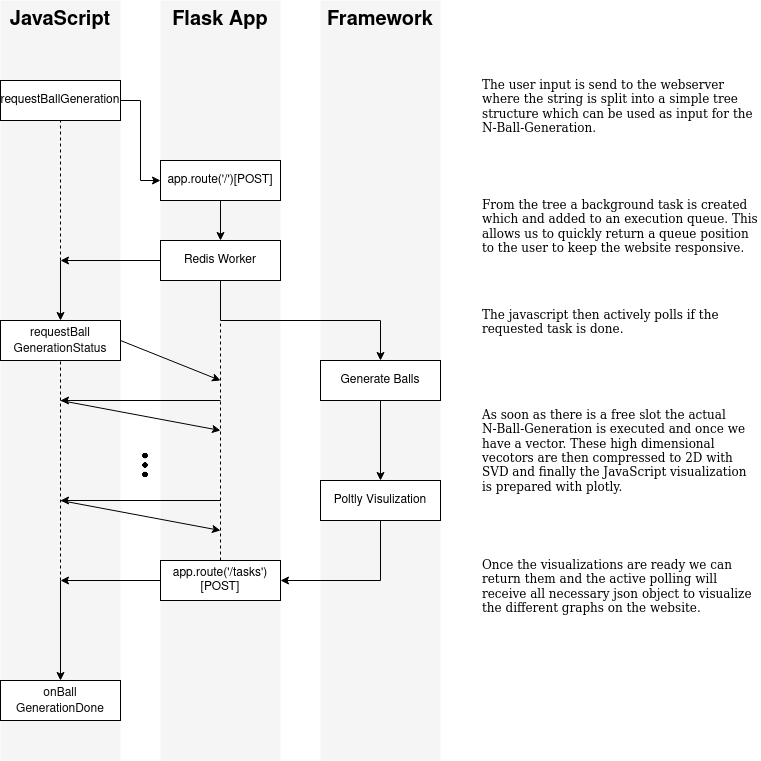
\includegraphics[width=\textwidth]{res/overview.png}
	\caption{architecture overview}
	\label{fig:overview}
\end{figure}

To get the results back to the user without the need to reload or redirect on the website we are using asynchronous AJAX requests. As soon the user either submits his input form or a file we send an AJAX request to the Web server which is immediately returned along with information of the task ID that the user has been assigned as well as which task queue this task resides in. With these two pieces of information, the web client can then periodically request to get a status update on the progress of his task. This update request is answered with its current queue position or once a task is completed with the results of our plotly visualization. The realization results are passed back as a JSON file which will be parsed in the JavaScript and passed into a JavaScript plotly instance allowing us to display the different graphs.

\subsection[Flask]{Flask\textsuperscript{\hyperref[Oliver]{(2)}}}

\label{sec::flask}
In order to provide an easily accessible interactive demonstration, visualization, and debugging tool we choose the medium of a website. As the original N-Ball embedding is implemented in Python, Flask was chosen as a web framework.  Flask is a Python based micro-framework and as such does not require any additional libraries and is readily available through the python package manager. 
As is convention with a Flask application we provide HTML templates in the template folder. These templates are just the basic HTML skeleton which defines where and in which order different graphs, input fields, and text fields will be inserted on the website. The basic formatting is done through the CSS bootstrap framework. We further extend on this with our own CSS file which can be found under \textit{templates/static/css} along with the JavaScript code under \textit{templates/static/js}. 


\subsection[Redis]{Redis\textsuperscript{\hyperref[Oliver]{(2)}}}
\label{sec::redis}
For every input, the system needs to generate the corresponding ball embeddings, save each step in the construction process, reduce the dimension of the embedding down to two dimensions for visualization and resolve to overlap that results from the dimensionality reduction. Depending on the size of the input tree this process can take anywhere from a few seconds to a few minutes. With a naïve implementation, the Web server would simply do all of these tasks before sending back the response to the user. This would not only leave the user waiting with no feedback but even more importantly the server would not be reachable at all during that time frame for other users. While works well for a single user it is obviously unacceptable for a publicly available website. We need to make sure that a large request will not block the Web server for everybody else for minutes, possibly even hours. Therefore we need to decouple the serving of the website from the actual computation of the ball embeddings. This is done by using a task queue.
We chose to use a commonly used task queue named Redis. This allows us to create a task queue, so when the user requests the computation of a ball embedding we add it to the task queue and immediately return to the user to tell him that we received his request and that he has been placed into the task queue. Once the task is complete the results can be sent to the user's browser through AJAX without the need to refresh or redirect the website. This allows for seamless display of the results. While the website will return immediately and give the user adequate feedback this still allows a single user to effectively block the queue. As he places a large request once the Web server starts computing this task it will not work on tasks that have been requested later. In order to keep the website's response time for small requests low, we introduced a second high priority queue that is reserved for small to moderate input sizes to ensure that users they want to experiment with the service will not be blocked by a single large request.
\begin{center}
	
	
	\begin{tabular}{c}
		\begin{lstlisting}
		r = redis.Redis()
		q_high = Queue("high", connection=r)
		q_low  = Queue("low", connection=r)  
		\end{lstlisting}
	\end{tabular}
\end{center}

\subsection[Plotly]{Plotly\textsuperscript{\hyperref[Joanna]{(3)}}} \label{sec::plotly}
Many different graphs were introduced to the web application to fully present N-Balls embeddings and help the user understand the functionality and the concept of it. A valuable tool, on which we based our figure visualizations, was the open-source library Plotly. It helped us to present data in many different forms using the Python language. It provided us with the means necessary to create scatter plots, shapes, annotations, tree plots as well as was a base for the interactive animated plot, which showed the work of the N-Ball embedding tree creation algorithm. In the end, leaving the user with a possibility to observe trees with different viewpoint as well as examine the construction process. Not only visualizations are showing the concept and algorithm behind but also, they are a useful tool to see if an inputted tree is correct and there are no structural problems with it. Plotly provides the graphical part of the application by allowing to present data/structures with different shapes and colors. Moreover, the library brings the graph management tools like zooming in/out. Once the plots will be generated in python with the use of Plotly they are serialized to JSON string to further be transferred to JavaScript which will manage its location and size on the website. 


\subsubsection{Paths tree}
After obtaining every keyword with its path, we combined them creating the forest of paths trees. The graph is focused on showing the user the structure and origins of the words. The clauses "is" and "is not" will indicate to which tree the word is belonging.


\begin{figure}[H]
	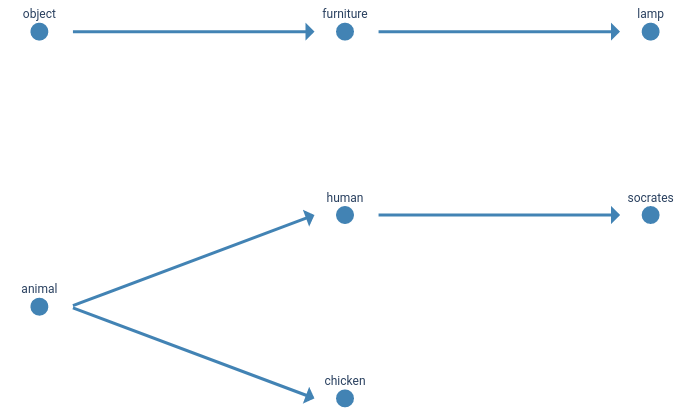
\includegraphics[width=\textwidth]{res/tree_forest.png}
	\caption{forest of words-paths trees plot}
	\label{fig:tree_forest}
\end{figure}


\subsubsection{N-Ball tree}

In the input, the algorithm receives the list of balls objects. They contain the location of the ball as well as its radius and label. With this information, the balls are transferred to the graph to show the relations between them.

\begin{figure}[H]
	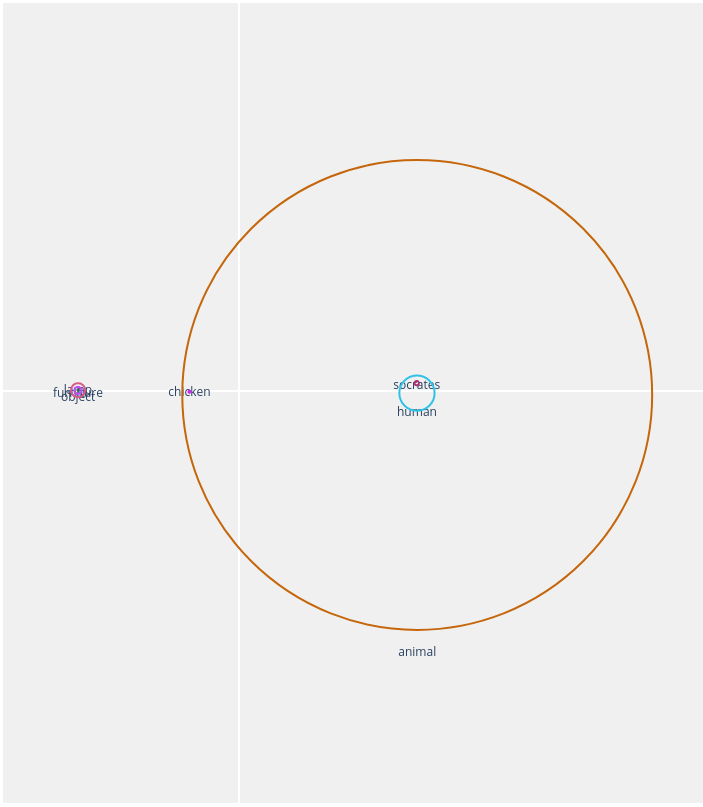
\includegraphics[width=\textwidth]{res/balls_graph.png}
	\caption{N-ball embeddings tree plot}
	\label{fig:balls_graph}
\end{figure}


\subsubsection{N-Ball tree animation}

Our animation is triggered by two buttons: "Next step", "Previous step". It is based on the same algorithm as the generation of N-Ball tree. With the difference that in this graph the animation algorithm will generate the same amount of N-Ball tree graphs as the amount of the steps of the balls generation algorithm took.  Therefore the received input for plots generation is a list of steps where every step contains a list of balls with its arguments.

We can distinguish different stages of ball creation:
\begin{itemize}
	\item initialize: prints the new ball to the plot.
	\item  contain: changes the position of the balls in relation to each other that one ball will be contained in another
	\item  separate: changes th position of the balls in relation to each other that the balls will be separated and will not contain each other
\end{itemize}

\begin{figure}[H]
	\begin{tabular}{cc}
		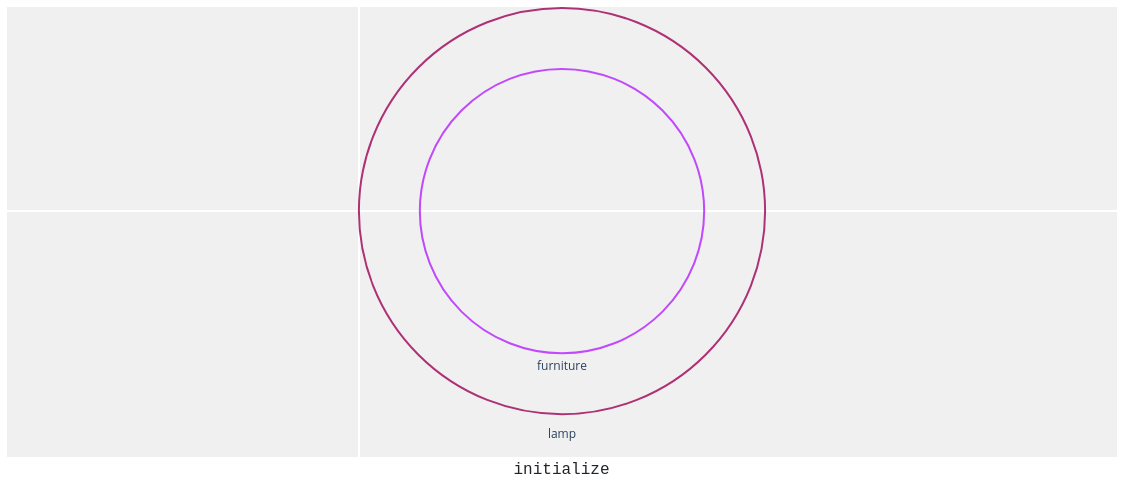
\includegraphics[width=55mm]{res/animation1.png} & 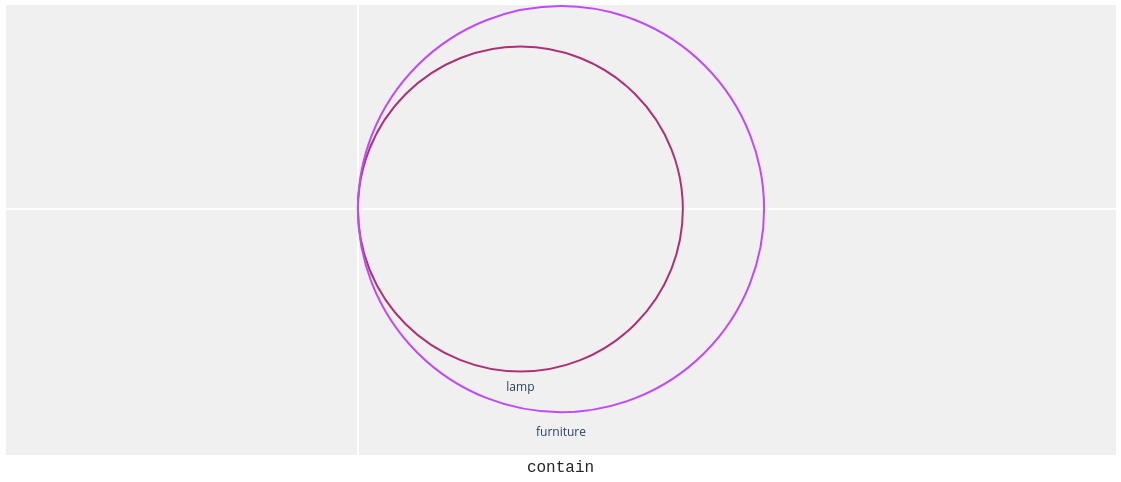
\includegraphics[width=55mm]{res/animation2.png} \\
		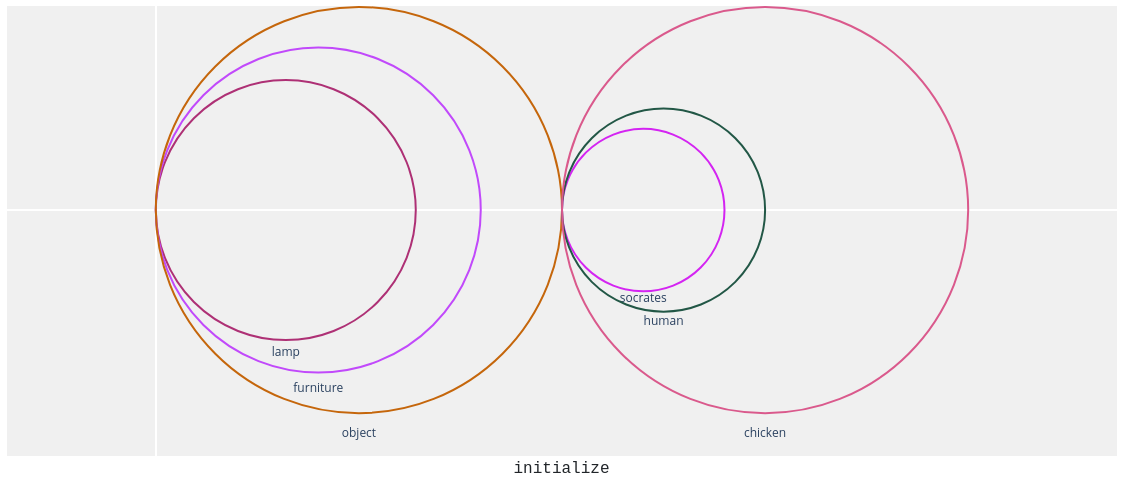
\includegraphics[width=55mm]{res/animation3.png} & 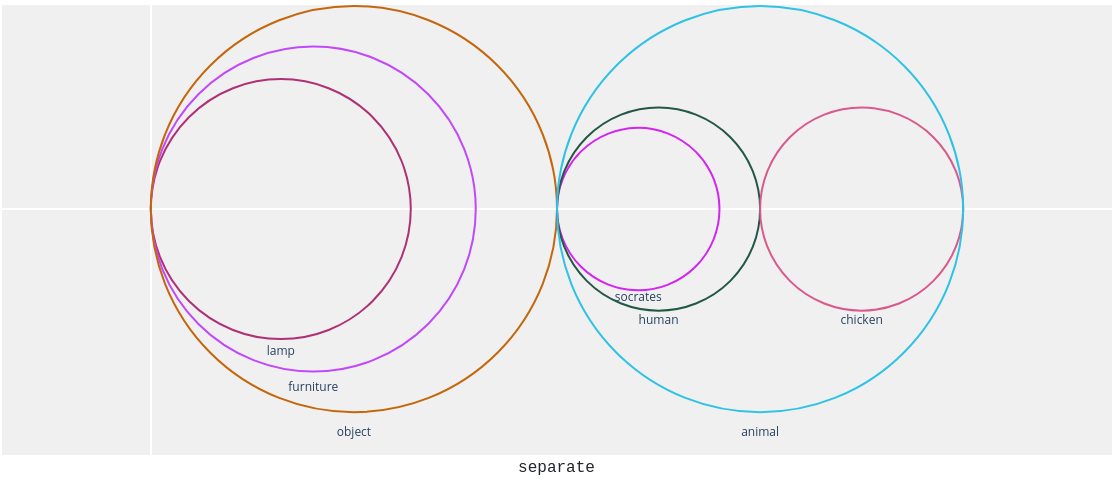
\includegraphics[width=55mm]{res/animation4.png} \\
	\end{tabular}
	\caption{N-Ball tree animation plot. Step 3,4, }
	\label{fig:animation}
\end{figure}

\subsection{Word sense exploration}
The initial scope of the project was planning to extract the tree structure that is needed to compute the N-Ball embedding from wordnet. WordNet is a database that collects semantic relationships between English words. The user would have simply given a list of input words that he wishes to explore and we would get all possible connections between these words from WordNet. 
Right away one issue arises as many words in the English language change their meaning depending on the context they are used in. For example the word tank can be used to describe a fillable container or the armored vehicle used in most modern wars. To resolve this ambiguity WordNet attaches a word sense notation to each word. In our example tank.n.01 and tank.n.02 as well as many more. Every entry will now uniquely respond to one word sentence of the word tank. This notation uses .n to denote nouns and .v to denote verbs. After this separation it simply enumerates all existing word sentences. Now that the meaning of each entry is fixed WordNet can assign meaningful relationships between these unique entities. 

However it might confuse the user that he provided a single word tank but the system presents him with multiple versions of the same word. To make this more understandable we build a word sense Explorer that shows the user which word sentences exist for every input word. Further we would give a definition of the selected word sense along with a single branch going back from this entity up to the root node that is being visualized.

\begin{figure}[H]
	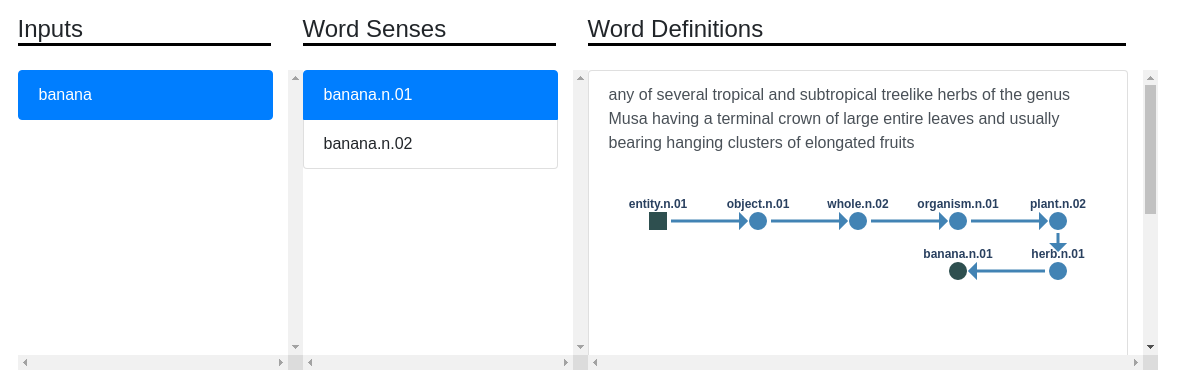
\includegraphics[width=\textwidth]{res/word-sense.png}
	\caption{words senses Explorer}
	\label{fig:word-sense}
\end{figure}



Later during the project it was decided to shift the focus of the project towards visual debugging and this feature was discontinued.

\section[User Interaction]{User Interaction\textsuperscript{\hyperref[Joanna]{(3)}}}

\subsection{Page overview}
The page was created in a simple and intuitive manner so the user can have a clear intuition of the functionalities as well as understand its purpose. The color scheme was chosen based on university colors. 

Page is divided into: 
\begin{itemize}
	\item header with logo, title and contact button,
	\item input box with two methods of submission,
	\item main body with the generated results.
\end{itemize}


\begin{figure}[H]
	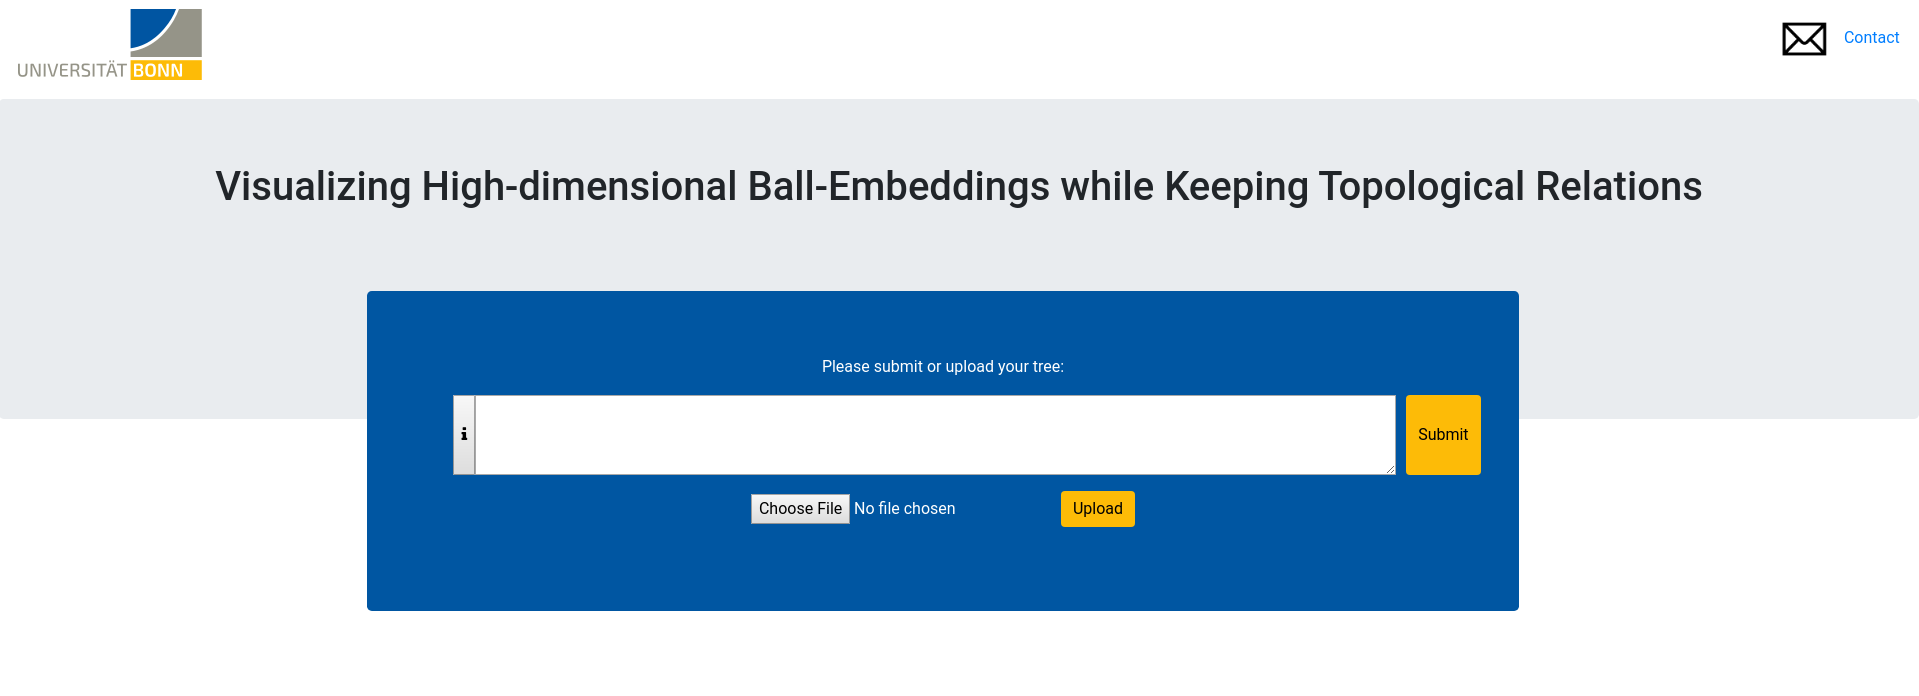
\includegraphics[width=\textwidth]{res/page.png}
	\caption{web page overview}
	\label{fig:page}
\end{figure}


\subsubsection{Contact}
We provided the contact possibility if there are any questions or remarks. Contact button transfers automatically to the mail service with pre-filled mail address.

\subsubsection{Info}
Clicking the little button with "i" icon, close to a text box, triggers the opening of the pop up which includes the explanatory information about the input and its example in a clear way that the user knows how to construct his/her own tree. 

\subsection{Input}
The application provides two ways for input. Its purpose is to ease the user interaction and give the option depending on the size of the query. 

\begin{itemize}
	\item Text box: user writes manually the input. Created with the thought of small inputs as well as dedicated to page exploration. Text box can accommodate long strings however its main purpose is small query testing. The generation of the output is followed after providing the proper input and clicking on the submit button next to the text box.
	\item  File upload: function dedicated to pre-written texts, big queries as well as additional information like users own ball embeddings. Designed with the thought to ease the process of creation of the query and faster tree structure testing. Users can use the editor of their own choice for flexibility and then upload files in the text format as well as JSON. 
\end{itemize}


\subsection{Output}
After input submission website shows three different plots. While the graphs calculating and generation take time depending on the size of the query, user is provided with waiting animation to indicate the process. 

\begin{figure}[H]
	\centering
	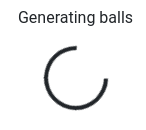
\includegraphics[scale=0.5]{res/waiting.png}
	\caption{waiting annimation}
	\label{fig:waiting}
\end{figure}


Plots provide user with different intake and presentation of the inputted tree:
\begin{itemize}
	\item Path tree: shows a forest of trees from a structural perspective. User can have an overview of what are exact word paths and how they interact with each other.
	\item N-Ball tree: shows the ball embeddings and their relation between each other.
	\item N-Ball tree animation: shows the process of ball embeddings creation. User is provided with two buttons to move to the next and previous step of the application as well as is provided with titles explaining the step.	
\end{itemize}

All the plots are zoomable with the scrooll wheel. 
For more information about the plots look to section \ref{sec::plotly}.
